\fenicschapter{Cerebrospinal Fluid Flow}
              {Cerebrospinal Fluid Flow}
              {Susanne Hentschel, Svein Linge, Emil Alf L{\o}vgren and Kent-Andre Mardal}
              {hentschel}

%Write a short introduction to your chapter here. Explain the purpose
%of the chapter and include a brief outline. Remember to index important
%terms and use citations.~~\cite{Cia78}

%------------------------------------------------------------------------------

\DefineVerbatimEnvironment{code}{Verbatim}{frame=single,rulecolor=\color{blue}, fontsize=\scriptsize, tabsize=2}

\section{Medical Background}

The cerebrospinal fluid (CSF) is a clear water-like fluid which occupies the so-called subarachnoid space (SAS) surrounding the brain and the spinal cord, and the ventricular system within the brain. The SAS is composed of a cranial and a spinal part, bounded by tissue layers, the dura mater as outer boundary and the pia mater as internal boundary. The cranial and the spinal SAS are connected by an opening in the skull, called the foramen magnum\index{foramen magnum}. One important function of the CSF is to act as a shock absorber and to allow the brain to expand and contract as a reaction to the changing cranial blood volume throughout the cardiac cycle. During systole the blood volume that enters the brain through the arterial system exceeds the volume that leaves the brain through the venous system and leads therefore to an expansion of the brain. The opposite effect occurs during diastole, when the blood volume in the brain returns to the starting point. Hence the pulse that travels through the blood vessel network is transformed to a pulse in the  CSF system, that is damped on its way along the spinal canal. \index{spinal canal} 

\index{cerebrospinal fluid}
\index{CSF}
\index{subarachnoid space}
\index{SAS}


\begin{figure}\begin{center}

\includegraphics[width=100mm]{chapters/haughton/eps/chiara_about.eps} 
\caption{Illustration of the cerebrospinal fluid system in a the normal case and with Chiari I malformation and syringomyelia (FIXME get permission to use this, found 
\emp{http://www.chiariinstitute.com/chiari\_malformation.html})}
\label{fig:anatomy}
\end{center}\end{figure}




The left picture in Figure \ref{fig:anatomy} shows the CSF and the main structures in the brain of a healthy individual. In about 0.6\% of the population the lower part of the cerebellum occupies parts of the CSF space in the upper spinal SAS and obstructs the flow. This so-called Chiari I malformation \index{Chiari I malformation} (or Arnold-Chiari malformation) (Milhorat et al. \cite{Milhorat1999}) is shown in the right picture in Figure \ref{fig:anatomy}. A variety of symptoms is related to this malformation, including headache, abnormal eye-movement, motor or sensor-dysfunctions, etc. If the malformation is not treated surgically, the condition may become more severe and will eventually cause more serious neurological deterioration, or even lead to death. Many people with the Chiari I malformation develop fluid filled cavities within the spinal cord, \index{spinal cord} a disease called syringomyelia (Oldfield \cite{Oldfield1994}). The exact relation between the Chiari I malformation and syringomyelia is however not known. It is believed that obstructions, that is abnormal anatomies cause abnormal flow leading to the development of syringomyelia (Oldfield \cite{Oldfield1994}). Several authors have analyzed the relations between abnormal flow and syringomyelia development based on measurements in patients and healthy volunteers  (Heiss ~\cite{Heiss1999}, Pinna ~\cite{Pinna2000}, Hofmann ~\cite{Hofmann2000}, Haughton ~\cite{Haughton2003}). The mentioned studies also compare the dynamics before and after decompressive surgery. The latter is an operation, where the SAS lumen around the obstructed area is increased by removing parts of the surrounding tissue and bones (Milhorat and Bolognese \cite{Milhorat2003}). Control images taken some weeks or months after the intervention often show a reduction of the size of the cavity in the spinal canal and patients usually report improvement of their condition. In some cases, the syrinx disappeared completely after some months (Oldfield \cite{1994}, Pinna \cite{Pinna2000}, Heiss \cite{Heiss1999}).\\

The studies mentioned above are all based on a small amount of individuals characterized by remarkable variations. CFD simulations may help to test the initial assumptions in generalized settings. Gupta ~\cite{Gupta2009} and Roldan ~\cite{Roldan2008} demonstrated the usefulness of CFD to quantify and visualize CSF flow in patient specific cases in great detail. It is the purpose of this chapter to describe the implementation of such a CFD solver in \fenics\ and to compare the simulation results with results obtained from Star-CD. Note that the Navier-Stokes solvers are discussed in detail in Chapter ~\cite{NS-bench}.\\

\section{Mathematical Description}

We model the CSF flow in the upper spinal canal as a Newtonian fluid \index{Newtonian fluid} with viscosity and density similar to water under body temperature. In the presented experiments, we focus on the dynamics around the spinal cord. The tissue surrounding the fluid is modeled as impermeable and rigid throughout the cardiac cycle. To simulate CSF flow, we apply the Navier-Stokes \index{Navier-Stokes} equations for an incompressible Newtonian fluid,  
\begin{eqnarray*}
\rho \left(\frac{\partial \mathbf{v}}{\partial t} + (\mathbf{v}\cdot\nabla) \mathbf{v}\right) &=& -\nabla p + \mu \Delta \mathbf{v} + \mathbf{g}, \quad \in \Omega, \\ 
\nabla \mathbf{v} &=& 0, \quad \in \Omega, 
\end{eqnarray*}
with the variables as indicated in Table \ref{tab:entities}, and $g$, the body force, i.e., gravity. We kan eliminate gravity from the equation by assuming that the body force is balanced by the hydrostatic pressure. As a result, pressure describes only the dynamic pressure. For calculating the physical correct pressure, static pressure resulting from body forces has to be added. This simplification is however not true during sudden movements such as raising up.  

The coordinate system is chosen so that the tubular axis points downwards, resulting in  positive systolic flow and negative diastolic flow.  

\begin{table}\begin{minipage}{\textwidth}\begin{center}
    \begin{tabular}{ | c | c | c | c | c | }
    \hline
    Symbol & Meaning & Entity & Chosen Value & Reference Value\\ \hline\hline
	$\mathbf{v}$	& velocity variable & $\mathrm{ \frac{cm}{s}}$ & --- & $-1.3\pm 0.6 \ldots 2.4 \pm 1.4$ \footnote{Hofmann et al. ~\cite{Hofmann2000}; Maximum absolute anterior CSF flow in both directions from controls and patients at foramen Magnum} \\ 
	$p$		& pressure	variable & mmHg & --- & \ldots\\
	$\rho$	& density & $\mathrm{\frac{g}{cm^3}}$ & --- &0.993 \footnote{at $37^\circ$ C }\\ %\textcelsius
	$\mu$	& dynamic viscosity	&  $\mathrm{\frac{g s}{cm}}$ & --- & 0.0007\\
	$\nu$	& kinematic viscosity & $\mathrm{ \frac{cm^2}{s}}$ & $0.7 10^{-2}$ & $0.7 10^{-2}$ \\ 	\hline %$(\nu = \frac{\mu}{\rho})$
	$SV$	& stroke volume \footnote{CSF volume that moves up and down through cross section in the SAS during one cardiac cycle}	& $\mathrm{ \frac{ml}{s}}$& $0.27$  & $0.27$\footnote{Gupta et al. \cite{Gupta2009}} \\
	$HR$	& heart rate & $\mathrm{\frac{beats}{s}}$	& 1.17 & 1.17\\
	$A0$	& tube boundary	& $\mathrm{ cm^2}$ & $32$  & ---\\
	$A1$,$A2$	& area of inlet/outlet & $\mathrm{ cm^2}$ &$0.93$ & 0.8 \ldots 1.1 \footnote{Loth et al. ~\cite{Loth2001}; Cross sections at 20--40 cm from the foramen magnum.}  \\
    \hline
    $Re$    & Reynholds Number & -- & -- & ~70--200 \footnote{See more details in \ref{tab:Re_We}.}\\
    $We$    & Womersley Number & -- & -- & ~14--17 \\
    \hline
    \end{tabular}
	\label{tab:entities}
	\caption{Characteristic values and parameters for CSF flow modeling.}
\end{center}\end{minipage}\end{table}
% reference: http://www.thermexcel.com/english/tables/eau_atm.htm

\section{Numerical Experiments} 
\subsection{Implementation}
We refer to Chapter ~\cite{NS} for a complete description of the solvers
and schemes implemented. In this chapter we concentrate on the use of
these solvers in a few examples.  

The problem is defined in a separate python script and can be found in: \\
 \emp{fenics-bok/csf/code/FILENAME}. The main parts are presented below.
%FIXME

\paragraph{Mesh boundaries.}  The mesh boundaries at the inlet cross section, the outlet cross section, and the SAS boundaries are defined by the respective classes \emp{Top}, \emp{Bottom}, and \emp{Contour}. They are implemented as subclasses of \emp{SubDomain}, similarily to the given example of \emp{Top}.
\begin{code}
class Top(SubDomain):	
	def __init__(self, index, z_max, z_min):
		SubDomain.__init__(self)
		self.z_index = index
		self.z_max = z_max
		self.z_min = z_min
	
	def inside(self, x, on_boundary):
		return bool(on_boundary and x[self.z_index] == self.z_max)
\end{code}
To define the domain correctly, we override the base class' object function \emp{inside}. It returns a boolean evaluating if the inserted point \emp{x} is part of the sub domain. The boolean \emp{on\_boundary} is very useful to easily partition the whole mesh boundary to sub domains. 

Physically more correct would be to require, that the no slip condition is also valid on the outermost/innermost nodes of the inflow and outflow sections as implemented below:
\begin{code}
def on_ellipse(x, a, b, x_index, y_index, x_move=0, y_move=0):
	x1 = x[x_index] - x_move
	x2 = x[y_index] - y_move
	return bool( abs((x1/a)**2 + (x2/b)**2 - 1.0 ) < 10**(-6) )
\end{code}
The vectors describing the ellipses of the cord and the dura in a cross section with the corresponding axes are required. The global function \emp{on\_ellipse} checks if \emp{x} is on the ellipse defined by the x-vector \emp{a} and the y-vector \emp{b}. The variables \emp{x\_move} and \emp{y\_move} allow to define an eccentric ellipse. 

Defining the inflow area at the top with excluded mantle nodes is done as follows below, the outflow area at the bottom is defined analogously.

\begin{code}
class Top(SubDomain):	#bc for top
	def __init__(self, a2_o, a2_i, b2_o, b2_i,  x_index, y_index, z_index, z_max, x2_o_move=0,\
				 y2_o_move=0, x2_i_move=0, y2_i_move=0):
		SubDomain.__init__(self)
		self.x_index = x_index
		self.y_index = y_index
		self.a2_o = a2_o
		self.a2_i = a2_i
		self.b2_o = b2_o
		self.b2_i = b2_i
		self.z_index = z_index
		self.z_max = z_max
		self.x2_o_move = x2_o_move
		self.x2_i_move = x2_i_move
		self.y2_o_move = y2_o_move
		self.y2_i_move = y2_i_move

	def inside(self, x, on_boundary):
		return bool(on_boundary and abs(x[self.z_index] - self.z_max) <10**(-6) \
                       and not on_ellipse(x, self.a2_o, self.b2_o, self.x_index,  \
                           self.y_index, self.x2_o_move, self.y2_o_move )\
                       and not on_ellipse(x, self.a2_i, self.b2_i, self.x_index, \ 
                           self.y_index, self.x2_i_move, self.y2_i_move ) ) 
\end{code}

The underscores \emp{o} and \emp{i} represent the outer and inner ellipse respectively. The numbering with \emp{2} distinguishes the sub domain at the top from that at the bottom that may be defined differently. The details of how different problems can easily be defined in separate classes can be found in:
\emp{src/mesh\_definitions/}. %FIXME

\paragraph{Inflow and outflow pulse.} According to Gupta et al. ~\cite{Gupta2009}, a volume of 0.27 ml is transported back and forth through the spinal SAS cross sections during the cardiac cycle. For the average human, we assumed a heart rate of 70 beats per minute. Furthermore, we defined the cross sectional area to be 0.93 $\mathrm{cm^2}$, which matches the segment from 20 to 40 cm down from the foramen magnum (Loth et al ~\cite{Loth2001}). In this region of the spinal canal, the cross sectional area varies little. In addition, the dura and the cord shape resemble a simple tube more than in other regions. According to Oldfield et al. ~\cite{Oldfield1994}, syrinxes start at around 5 cm below the foramen magnum and reach down up to 28 cm below the foramen magnum. 

Further, we define a velocity pulse on the inflow and outflow boundaries and since we are modeling incompressible flow between rigid impermeable boundaries, we must have equal inflow and outflow volume at all times. The pulse values in these boundary cross sections were set equal in every grid point, and scaled to match the volume transport of 0.27 ml. 

\begin{figure}\begin{center}
\includegraphics[width = 0.5\textwidth]{chapters/haughton/eps/sin_pulse.eps}
\caption{Two different flow pulses.}
\label{fig:sin_pulse}. 
\end{center}\end{figure}

Smith et al. \cite{Smith2006} introduced a function describing the varying blood pressure in a heart chamber(see Figure \ref{fig:sin_pulse}). With some adjustment and additional parameters, the function was adapted to approximate the CSF flow pulse. The systole of the pulse function is characterized by a high amplitude with a short duration while the negative counter movement has a reduced amplitude and lasts considerably longer. 
The global function for defining the pulse is:
\begin{code}
def get_pulse_input_function(V, z_index, factor, A, HR_inv, HR, b, f1):
	two_pi = 3.4 * pi
	rad = two_pi /HR_inv	
	v_z = "factor*(-A*(exp(-fmod(t,T)*rad)*Ees*(sin(-f1*fmod(t,T)*rad)-vd)\
          -(1-exp(-factor*fmod(t,T)*rad))*p0*(exp(sin(-fmod(t,T)*rad)-vd)-1))-b)"
	vel = None
	if z_index == 0:
		vel = (v_z, "0.0", "0.0")
	elif z_index ==1:
		vel = ("0.0", v_z, "0.0")
	elif z_index ==2:
		vel = ("0.0", "0.0", v_z)

	class Pulse(Function):
		cpparg = vel
		print vel
		defaults = {"factor":factor, "A":A, "p0":1, "vd":0.03, "Ees":50, "T":HR_inv, "HR":HR,\
                     "rad":rad, "b":b, \emp{f1}:f1}

	return Pulse(V)
\end{code}
To define the necessary parameters in the initialization, the following lines are required.
\begin{code}
self.A = 2.9/16	# scale to get max = 2.5 and min = -0.5 for f1 = 1
self.factor = self.flow_per_unit_area/0.324		
self.v_max = 2.5 * self.factor
self.b = 0.465 	# translating the function "down"
self.f1 = 0.8
\end{code}

The boundary condition \emp{Pulse} is defined as a subclass of \emp{Function}, that enables parameter dependencies evaluated at run time. To invoke an object of \emp{Pulse}, the global function \emp{get\_pulse\_input\_function} has to be called. The function input contains all necessary constants to define the pulse function, scaled to cardiac cycle and volume transport. The index \emp{z\_index} defines the coordinate of the tubular direction. The Velocity Function Space \emp{V} is a necessary input for the base class \emp{Function}. 




\paragraph{Initialization of the problem.} The initialization of the class \emp{Problem} defines the mesh with its boundaries and provides the necessary information for the Navier--Stokes solvers. The mesh is ordered for all entities and initiated to compute its faces.


The values \emp{z\_min} and \emp{z\_max} mark the inflow and outflow coordinates along the tube's length axis. As mentioned above, the axis along the tube is indicated by \emp{z\_index}. If one of the coordinates or the z-index is not known, it may help to call the mesh in viper \emp{unix>viper meshname.xml}. Typing \emp{o} prints the length in x, y and z direction in the terminal window. Defining \emp{z\_min}, \emp{z\_max} and \emp{z\_index} correctly is important for the classes that define the boundary domains of the mesh \emp{Top}, \emp{Bottom} and \emp{Contour}. As we have seen before, \emp{z\_index} is necessary to set the correct component to the non-zero boundary velocity. 

Exterior forces on the Navier--Stokes flow are defined in the object variable \emp{f}. We have earlier mentioned that gravity is neglected in the current problem so that the force function \emp{f} is defined by a constant function \emp{Constant} with value zero on the complete mesh.

After initializing the sub domains, \emp{Top}, \emp{Bottom} and \emp{Contour}, they are marked with reference numbers attributed to the collection of all sub domains \emp{sub\_domains}. 

To see the most important effects, the simulation was run slightly longer than one full period. A test verified that the initial condition of zero velocity in all points is sufficiently correct and leads to a good result in the first period already. Besides maximum and minimum velocities, it includes the transition from diastole to systole and vice versa.  With the given time step length, the simulation is very detailed in time.    
\begin{code}
def __init__(self, options):
	ProblemBase.__init__(self, options)
	#filename = options["mesh"]
	filename = "../../data/meshes/chiari/csf_extrude_2d_bd1.xml.gz"
	self.mesh = Mesh(filename)
	self.mesh.order()
	self.mesh.init(2)

	self.z_max = 5.0	# in cm
	self.z_min = 0.0	# in cm
	self.z_index = 2
	self.D = 0.5 		# characteristic diameter in cm

	self.contour = Contour(self.z_index, self.z_max, self.z_min)
	self.bottom = Bottom(self.z_index, self.z_max, self.z_min)
	self.top = Top(self.z_index, self.z_max, self.z_min)

    # Load sub domain markers
	self.sub_domains =  MeshFunction("uint", self.mesh, self.mesh.topology().dim() - 1)

	# Mark all facets as sub domain 3
	for i in range(self.sub_domains.size()):
		self.sub_domains.set(i, 3)

	self.contour.mark(self.sub_domains, 0)
	self.top.mark(self.sub_domains, 1)
	self.bottom.mark(self.sub_domains, 2)

    # Set viscosity 
	self.nu = 0.7 *10**(-2) # cm^2/s  

    # Create right-hand side function
	self.f = Constant(self.mesh, (0.0, 0.0, 0.0))
	n = FacetNormal(self.mesh)

    # Set end-time
	self.T = 1.2* 1.0/self.HR
	self.dt = 0.001
\end{code}


Increasing the time step length usually speeds up the calculation of the solution. As long as the CFL number with the maximum velocity $v_{max}$, time step length $dt$ and minimal edge length $h_{min}$ is smaller than one $(CFL = \frac{v_{max} dt}{h_{min}} < 1)$, the solvers should (!!!) converge. For too small time steps it can however lead to an increasing number of iterations for the solver on each time step.  As a characterization of the fluid flow, the Reynholds number $(Re = \frac{v_c l}{\nu})$ was calculated with the maximum velocity $v_c$ at the inflow boundary and the characteristic length $l$ of the largest gap between outer and inner boundary. Comparison of Reynholds numbers for different scenarios  can be found in Table \ref{tab:Re_We}. 


The area of the mesh surfaces and the mesh size can be found as follows. 
\begin{code}
self.h = MeshSize(self.mesh)
self.A0 = self.area(0)
self.A1 = self.area(1)
self.A2 = self.area(2)

def area(self, i): 
	f = Constant(self.mesh, 1)
	A = f*ds(i)
	a = assemble(A, exterior_facet_domains=self.sub_domains)
	return a 
\end{code}



\paragraph{Object Functions.} Being a subclass of \emp{ProblemBase}, \emp{Problem} overrides the object functions \emp{update} and \emp{functional}. The first ensures that all time--dependent variables are updated for the current time step. The latter prints the maximum values for pressure and velocity. The normal flux through the boundaries is defined in the separate function \emp{flux}.
\begin{code}
def update(self, t, u, p):
	self.g1.t = t
	self.g2.t = t
	pass
def functional(self, t, u, p):
	v_max = u.vector().norm(linf)
	f0 = self.flux(0,u)
	f1 = self.flux(1,u)
	f2 = self.flux(2,u)
	pressure_at_peak_v = p.vector()[0]

	print "time ", t 
	print "max value of u ", v_max
	print "max value of p ", p.vector().norm(linf)
	print "CFL = ", v_max * self.dt / self.h.min()
	print "flux through top ", f1
	print "flux through bottom ", f2

	# if current velocity is peak
	if v_max >  self.peak_v:
		self.peak_v = v_max
		print pressure_at_peak_v
		self.pressure_at_peak_v = pressure_at_peak_v

	return pressure_at_peak_v

def flux(self, i, u): 
	n = FacetNormal(self.mesh)
	A = dot(u,n)*ds(i)
	a = assemble(A, exterior_facet_domains=self.sub_domains)
	return a 
\end{code}

The boundary conditions are all given as Dirichlet conditions, associated with their velocity function space and the belonging sub domain. The additional functions \emp{boundary\_conditions} and \emp{initial\_conditions} define the respective conditions for the problem that are called by the solver. Boundary conditions for velocity, pressure and psi (???) are collected in the lists \emp{bcv}, \emp{bcp} and \emp{bcpsi}. 

\begin{code}
def boundary_conditions(self, V, Q):
	# Create no-slip boundary condition for velocity
	self.g0 = Constant(self.mesh, (0.0, 0.0, 0.0))
	bc0 = DirichletBC(V, self.g0, self.contour)

	# create function for inlet and outlet BC
	self.g1 = get_sine_input_function(V, self.z_index, self.HR, self.HR_inv, self.v_max)
	self.g2 = self.g1 

	# Create inflow boundary condition for velocity on side 1 and 2
	bc1 = DirichletBC(V, self.g1, self.top)
	bc2 = DirichletBC(V, self.g2, self.bottom)	

	# Collect boundary conditions
	bcv = [bc1, bc0, bc2]
	bcp = []
	bcpsi = []

	return bcv, bcp, bcpsi

def initial_conditions(self, V, Q):

	u0 = Constant(self.mesh, (0.0, 0.0, 0.0))
	p0 = Constant(self.mesh, 0.0)

	return u0, p0
\end{code}


\paragraph{Running.}
Applying the "Chorin" solver, the Problem is started by typing :

\emp{unix>./ns csf\_flow chorin}. 

It approximates the Navier--Stokes equation with Chorin's method. The progress of different simulation steps and results, including maximum calculated pressure and velocity per time step, are printed out on the terminal. In addition, the solution for pressure and velocity are dumped to a file for each (by default?) time step. Before investigating the results, we introduce how the mesh is generated. 


\subsection{Example 1. Simulation of a Pulse in the SAS.} 
In the first example we represent the spinal cord and the surrounding dura mater as two straight cylinders.  These cylinders can easily be generated by using NetGen ~\cite{netgen} or Gmsh ~\cite{gmsh}.  In NetGen meshes can be constructed by adding or subtracting geometrical primitives from each other. It also supports \dolfin\ mesh generation. Examples for mesh generation with NetGen can be found in \ldots. 

In Gmsh, constructing the basic shapes requires a more complex geometrical description, however it is easier to control how the geometry is meshed. The following code example shows the construction of a circular cylinder (representing the pia on the spinal cord) within an elliptic cylinder (representing the dura). The dura is defined by the ellipse vectors a=0.65 mm and b=0.7 mm in x and y direction respectively. The cord has a radius of 4 mm with its center moved 0.8 mm in positive x-direction  Since Gmsh only allows to draw circular or elliptic arcs for angles smaller than $pi$, the basic ellipses were constructed from four arcs each. Every arc is defined by the starting point, the center, another point on the arc and the end point. The value $lc$  defines the maximal edge length in vicinity to the point.

\begin{code}
lc = 0.04;
Point(1) = {0,0,0,lc};	// center point
//outer ellipses
a = 0.65;
b = 0.7;
Point(2) = {a,0,0,lc};	
Point(3) = {0,b,0,lc};	
Point(4) = {-a,0,0,lc};
Point(5) = {0,-b,0,lc};
Ellipse(10) = {2,1,3,3};
Ellipse(11) = {3,1,4,4};
Ellipse(12) = {4,1,5,5};
Ellipse(13) = {5,1,2,2};

// inner ellipses
move = 0.08; //"move" center
Point(101) = {move,0,0,lc};
c = 0.4;
d = 0.4;
Point(6) = {c+move,0,0,lc*0.2};
Point(7) = {move,d,0,lc};
Point(8) = {-c+move,0,0,lc};
Point(9) = {move,-d,0,lc};
Ellipse(14) = {6,101,7,7};
Ellipse(15) = {7,101,8,8};
Ellipse(16) = {8,101,9,9};
Ellipse(17) = {9,101,6,6};
\end{code}

The constructed ellipses are composed of separate arcs. To define them as single lines, the ellipse arcs are connected in line loops. 

\begin{code}
// connect lines of outer and inner ellipses to one
Line Loop(20) = {10,11,12,13};		// only outer
Line Loop(21) = {-14,-15,-16,-17};	// only inner
\end{code}
The SAS surface between cord and dura is then defined by the following command.
\begin{code}
Plane Surface(32) = {20,21};
\end{code}

To easily construct volumes, Gmsh allows to extrude a generated surface over a given length. 
\begin{code}
length = 5.0
csf[] = Extrude(0,0,length){Surface{32};};
\end{code}


Calling the .geo file in Gmsh
\emp{>unix Gmsh filename.geo}
shows the defined geometry. Changing to Mesh modus in the interactive panel and pressing \emp{3d} constructs the mesh. Pressing \emp{Save} will save the mesh with the .geo--filename and the extension \emp{msh}. For use in \dolfin, the mesh generated in Gmsh can be converted by applying the \dolfin\ converter.\\

\emp{unix>dolfin-convert mesh-name.msh mesh-name.xml}


\begin{figure}\begin{center}
\includegraphics[width=100mm]{chapters/haughton/eps/gmsh.eps}
\caption{Gmsh mesh.}
\label{fig:Gmsh_mesh}. 
\end{center}\end{figure}



\paragraph{Results}
The simulation results for an appropriate mesh (see verification below) can be found in Figure \ref{fig:case1}. The plots show the velocity component in tubular direction at at the mid cross section of the model. The flow profiles are taken at the time steps of maximum flow in both directions and during the transition from systole to diastole. For maximal systole, the velocities have two peak rings, one close to the outer, the other to the inner boundary. We can see sharp profiles at the maxima and bidirectional flow at the local minimum during diastole. 


\begin{figure}\begin{center}
\includegraphics[width=0.3\textwidth]{chapters/haughton/eps/pulse_f1_08_sysmax_nmb7.eps}
\includegraphics[width=0.3\textwidth]{chapters/haughton/eps/pulse_f1_08_sysdia_nmb18.eps}
\includegraphics[width=0.3\textwidth]{chapters/haughton/eps/pulse_f1_08_diamin1_nmb25.eps}
\caption{Case: Circular cord. The velocity in z-direction for the non-symmetric pulse at the time steps $t=0.07s, 0.18s, 0.25s$.}
\label{fig:case1}. 
\end{center}\end{figure}


\subsubsection{Comparing different solvers.}
For the first example, we applied the Chorin solver (WRITE ABOUT MODIFICATIONS WITH TOLERANCES!). For verifying the result, we also applied the solvers G2 and Uzawa. We picked an arbitrary point in the mesh to compare its pressure value at the time step of peak velocity. The results shown in Table \ref{tab:entities} reveal remarkable differences for \ldots Due to its simplicity with rather high accuracy, we have chosen the Chorin solver for further simulations.

\begin{table}\begin{center}
    \begin{tabular}{ | c | c | c | c |}
    \hline
    Solver & $p$ in Pa & $\mathbf{v}_{max}$ in cm/s  & $t$ in s \\ \hline\hline
	Chorin & 4.03 & 1.35 & 0.233 	\\ \hline
	G2	&	6.70 & 0.924 & 0.217	\\ \hline
	Uzawa	&	& 		&\\	
    \hline
    \end{tabular}
	\label{tab:solvers}
	\caption{The pressure at peak velocity in an arbitrary mesh cell for the different solvers.}
\end{center}\end{table}


\subsubsection{Verifying the mesh.}
In our case, the resolution in the cross section is more important than along the pipe. Gmsh allows to construct uniform meshes with a predefined number of layers in the main flow direction. With the unnatural boundary conditions of equal velocity throughout the inflow and outflow cross sections (plug flow), the correct velocity field develops between the pipe's ends. In the current section, we try to find out how long the pipe has to be, so that the mid--cross section represents the fully developed profile. Further, we know that there is a boundary layer close to the boundary, characterized by a steep velocity gradient. To capture the latter, we generated three mesh layers containing triangles of small edge size on the inner and the outer boundary. The distance of the layers was chosen, so that the edge length slightly increases for each layer. Starting from 10\% of the maximum edge length, for the first layer, the width of the second and the third layer was set to 30\% and 80\% of the maximum edge length. Comparisons of a mesh with and without boundary layers can be seen in Figure \ref{fig:boundary_layers}.


FIGUR EINFUEGEN

%\begin{figure}\begin{center}
%\includegraphics[width=0.3\textwidth]{chapters/csf_flow/eps/pulse_f1_08_sysmax_nmb7.eps}
%\includegraphics[width=0.3\textwidth]{chapters/csf_flow/eps/pulse_f1_08_sysdia_nmb18.eps}
%\includegraphics[width=0.3\textwidth]{chapters/csf_flow/eps/pulse_f1_08_diamin1_nmb25.eps}
%\caption{Case: Spinal SAS with (right) and without(left) boundary layers. The velocity in z-direction for the non-symmetric pulse at the time steps ??? $t=0.07, 0.18, 0.25$.}
%\label{fig:boundary_layers}. 
%\end{center}\end{figure}


To add mesh layers in Gmsh, copies for the elliptic arcs are scaled to gradually increase the maximum edge length. The code example below shows the creation of the layers close to the outer ellipse. The inner layers are created similarly.
\begin{code}
outer_b1[] = Dilate {{0, 0, 0}, 1.0 - 0.1*lc } { 
Duplicata{  Line{10}; Line{11}; Line{12}; Line{13}; } };
outer_b2[] = Dilate {{0, 0, 0}, 1.0 - 0.3*lc } { 
Duplicata{  Line{10}; Line{11}; Line{12}; Line{13}; } };
outer_b3[] = Dilate {{0, 0, 0}, 1.0 - 0.8*lc } { 
Duplicata{  Line{10}; Line{11}; Line{12}; Line{13}; } };
\end{code}
The single arcs are dilated separately since the arc points are necessary for further treatment. Remember that no arcs with angles smaller than $pi$ are allowed. Again we need a representation for the complete ellipses defined by line loops, as
\begin{code}
Line Loop(22) = {outer_b1[]};
\end{code}
that are necessary to define the surfaces between all neighboring ellipses similar to:
\begin{code}
Plane Surface(32) = {20,22};
\end{code}
Additionally, all Surfaces have to be listed in the Extrude command (see below).


To further adapt the mesh structure to the flow profile, we used the fact that the only non-zero velocity component is along the tubular length axis. The velocities of a cross sectional point only change along the tube, for cross sections close to the inflow and outflow boundaries but not in the region inbetween, where flow is fully developed. It is thus not required to have as dense nodes in the flow direction as required for the cross sections. For straight rigid pipes, we decided therefore to extrude the cross sectional mesh with a small number of layers per tube length. An additional advantage of this strategy is, that the meshes are uniform in every cross section. The layers can be specified during extrusion. Note that the list of extruded surfaces now contains six layers and the mid section.
\begin{code}
// Extrude
length = 5.0;		
layers = 30;		
csf[] = Extrude {0,0,length} {Surface{32}; Surface{33};
   Surface{34};Surface{35};Surface{36};Surface{37};Surface{38};Layers{ {layers}, {1} }; };
\end{code}

The complete code can be found in \ldots. The presented results were simulated on  meshes of length 5 cm with 30 layers in z-direction and three layers on the side boundaries.\\

Figure \ref{fig:z_layers} shows that extruded meshes result in smoother cross section images. 

Testing different numbers of layers  ....

%FIGUR EINFUEGEN
%\begin{figure}\begin{center}
%\includegraphics[width=0.3\textwidth]{chapters/csf_flow/eps/pulse_f1_08_sysmax_nmb7.eps}
%\includegraphics[width=0.3\textwidth]{chapters/csf_flow/eps/pulse_f1_08_sysdia_nmb18.eps}
%\includegraphics[width=0.3\textwidth]{chapters/csf_flow/eps/pulse_f1_08_diamin1_nmb25.eps}
%\caption{Case: Spinal SAS with (right) and without(left) layers in z-direction. The velocity in z-direction for the non-symmetric pulse at the time steps ??? $t=0.07s, 0.18s, 0.25s$.}
%\label{fig:z_layers}. 
%\end{center}\end{figure}




 

\subsection{Example 2. Simplified Boundary Conditions.} 

Many researchers apply the sine function as inlet and outlet boundary condition, since its integral is zero over one period. However, itss shape is not in agreement with measurements of the cardiac flow pulse (Loth et al. \cite{Loth2001}). To see the influence of the applied boundary condition for the defined mesh, we replace the more realistic pulse function with a sine, scaled to the same amount of volume transport per cardiac cycle. The code example below implements the alternative pulse function in the object function \emp{boundary\_conditions}. The variable \emp{sin\_integration\_factor} describes the integral of the first half of a sine.
\begin{code}
self.HR = 1.16 # heart rate in beats per second; from 70 bpm
self.HR_inv = 1.0/self.HR
self.SV = 0.27 
self.A1 = self.area(1)
self.flow_per_unit_area = self.volume_flow/self.A1
sin_integration_factor = 0.315
self.v_max = self.flow_per_unit_area/sin_integration_factor	
\end{code}
As before, we have a global function returning the sine as a Function - object, 
\begin{code}
def get_sine_input_function(V, z_index, HR, HR_inv, v_max):
	v_z = "sin(2*pi*HR*fmod(t,T))*(v_max)"
	vel = ["0.0", "0.0", "0.0"]
	vel[z_index] = v_z
	class Sine(Function):
		cpparg = tuple(vel)
		defaults = {'HR}:HR, \emp{v_max}:v_max, \emp{T}:HR_inv}		

	return Sine(V)
\end{code}
that is called instead of \emp{get\_pulse\_input\_function} in the function \emp{boundary\_conditions}:
\begin{code}
self.g1 = get_sine_input_function(V, self.z_index, self.factor, self.A, self.HR_inv, self.HR,\
                                  self.b, self.f1).
\end{code}



The pulse and the sine are sketched in Figure \ref{fig:sin_pulse}. Both functions are marked at the points of interest: maximum systolic flow, around the transition from systole to diastole and the (first, local) minimum. Results for sinusoidal boundary conditions are shown in Figure \ref{fig:case2} The shape of the flow profile is similar in every time step, only the magnitudes change. No bidirectional flow was discovered in the transition from positive to negative flow. Compared to the results received by the more realistic pulse function, the velocity profile generated from sinusoidal boundaries is more homogeneous over the cross section. 




\begin{figure}\begin{center}
\includegraphics[width=0.3\textwidth]{chapters/haughton/eps/sin_sysmax_nmb2.eps}
\includegraphics[width=0.3\textwidth]{chapters/haughton/eps/sin_sysdia_nmb4.eps}
\includegraphics[width=0.3\textwidth]{chapters/haughton/eps/sin_diamin_nmb6.eps}
\caption{Case: Circular Cord. The velocity in z-direction as response to a sine boundary condition for the time steps $t=0.2, 0.4, 0.6$.}
\label{fig:case2}. 
\end{center}\end{figure}





\subsection{Example 3. Cord Shape and Position.} 

According to ~\cite{Loth2001}, ~\cite{Alperin2006}, the present flow is inertia dominated, meaning that the shape of the cross section should not influence the pressure gradient. Changing the length of vectors describing the ellipse from
\begin{code}
c = 0.4;
d = 0.4;
\end{code}
to
\begin{code}
c = 0.32;
d = 0.5;
\end{code}
transforms the cross section of the inner cylinder to an elliptic shape with preserved area. The simulation results are collected in Figure \ref{fig:case3}. Comparisons showed that the pressure gradient was identical for the two cases, the different shape is however reflected in the flow profiles.


A further perturbation of the SAS cross sections was achieved by changing the moving of the center of the elliptic cord from
\begin{code}
move = 0.08;
\end{code}
to
\begin{code}
move = 0.16;
\end{code}
Also for this case the pressure field was identical, with some variations in the flow profiles.



\begin{figure}\begin{center}
\includegraphics[width=0.3\textwidth]{chapters/haughton/eps/pulse_f1_08_elliptic_sysmax_nmb7.eps}
\includegraphics[width=0.3\textwidth]{chapters/haughton/eps/pulse_f1_08_elliptic_sysdia_nmb18.eps}
\includegraphics[width=0.3\textwidth]{chapters/haughton/eps/pulse_f1_08_elliptic_diamin1_nmb25.eps}
\caption{Case: Elliptic cord. The velocity in z-direction for the non-symmetric pulse at the time steps $t=0.07s, 0.18s, 0.25s$.}
\label{fig:case3}. 
\end{center}\end{figure}



\begin{figure}\begin{center}
\includegraphics[width=0.3\textwidth]{chapters/haughton/eps/pulse_f1_08_elliptic_eccentric_sysmax_nmb7.eps}
\includegraphics[width=0.3\textwidth]{chapters/haughton/eps/pulse_f1_08_elliptic_eccentric_sysdia_nmb18.eps}
\includegraphics[width=0.3\textwidth]{chapters/haughton/eps/pulse_f1_08_elliptic_eccentric_diamin1_nmb25.eps}
\caption{Case: Translated elliptic cord. The velocity in z-direction for the non-symmetric pulse at the time steps $t=0.07s, 0.18s, 0.25s$.}
\label{fig:case3b}. 
\end{center}\end{figure}


\subsection{Example 4. Cord with Syrinx.} 
\begin{figure}\begin{center}
\includegraphics[width=0.3\textwidth]{chapters/haughton/eps/pulse_syrinx_f1_08_syrinx05_sysmax_nmb7.eps}
\includegraphics[width=0.3\textwidth]{chapters/haughton/eps/pulse_syrinx_f1_08_syrinx05_sysdia_nmb18.eps}
\includegraphics[width=0.3\textwidth]{chapters/haughton/eps/pulse_syrinx_f1_08_syrinx05_diamin1_nmb25.eps}
\caption{Case: Enlarged cord diameter. The velocity in z-direction for the non-symmetric pulse at the time steps $t=0.07s, 0.18s, 0.25s$.}
\label{fig:case4}
\end{center}\end{figure}

Syrinxes expand the cord so that it occupies more space of the spinal SAS. Increasing the cord radius from 4 mm to 5 mm \footnote{which equals to set the variables c and d in the geo-file to 0.5} decreases the cross sectional area by almost one third to 0.64 $\mathrm{cm^2}$. The resulting flow is shown in Figure \ref{fig:case4}. Apart from the increased velocities, we see bidirectional flow already at t = 0.18 and at t=0.25 as before. The fact that diastolic back flow is visible at t = 0.18, shows that the pulse with its increased amplitude travels faster. 

\begin{table}\begin{center}
    \begin{tabular}{ | c | c | c | c | c |}
    \hline
    Problem & $D$ \footnote{Characteristic length; $D=\sqrt(A/\pi)$, A being the inflow and outflow area} in cm & $\mathbf{v}_{max}$\footnote{at inflow and outflow boundary.} in cm/s  & $Re$ & $We$ \\ \hline\hline
	Example 1 	&	0.54 & 2.3 & 177 & 17	\\ \hline
	Example 2	&	0.54 & 0.92 & 70 & 17	\\ \hline
	Example 4	&	0.45 & 3.2 	& 205 & 14	\\ \hline
    \end{tabular}
	\label{tab:Re_We}
	\caption{Characteristic values for the examples 1, 2 and 3.}
\end{center}\end{table}

Comparing Reynholds and Womersly numbers shows a clear differene for the above described examples 1, 2 and 3. Example 2 is marked by a clearly lower maximum velocity at inflow and outflow boundary that leads to a rather low Reynholdsnumber. Due to the different inflow and outflow area, Example 4 has a lower Womerley number, leading to an elevated maximum velocity at the boundary and clearly increased Reynholds number. These numbers help to quantify the changes introduced by variations in the model. For the chosen model, the shape of the pulse function at the boundary condition as well as the cross sectional area have great influence on the simulation results. As earlier shown by Loth et al. \cite{Loth2001}, altering the shape of the cross sections does not seem to influence the flow greatly.
%\subsection{Example 5. Flow Around in a Patient-Specific Geometry.} 


